%!LW recipe=latexmk (latexmkrc)

\documentclass[10pt,aspectratio=169]{beamer}

\usepackage{amsmath}
\usepackage{amssymb}
\usepackage{mathtools}
\usepackage{amsthm}

\usepackage{bibentry}
\usepackage[backend=biber,style=ieee, citestyle=authoryear]{biblatex}


\bibliography{bibliography.bib}

\usetheme{moml}

\title[Learning Rate Schedules]{Learning Rate Schedules}
\subtitle{Deep Learning Research Kitchen}
\author[R. Uhrich]{Robin Uhrich}
\institute{}
% \titlegraphic{%
% 
%     % \includegraphics[width=0.3\linewidth]{graphics/UT_WBMW_Rot_RGB.pdf}%
%     \hspace{1em}%
% 
%     \includegraphics[width=0.3\linewidth]{graphics/imprs-is-logo.pdf}%
% }
\date[06.06.2024]{June 6, 2024}

% YouTube Links
\def\baselink{https://youtu.be/yQapprW_sZU}
\def\timelink#1{\baselink&t=#1}


\begin{document}

    \begin{frame}[plain]
        \titlepage
    \end{frame}

    \begin{darkframe}
        \frametitle{Outline}
        \begin{enumerate}
            \item Background - Why do we schedule learning rates in DL?
            \item Which LR schedules are used in practice?
            \item Experiments
            \item Scheduling other Hyperparameter
            \item Conclusion
        \end{enumerate}
    \end{darkframe}

    \begin{darkframe}
        \frametitle{Outline}

        \begin{enumerate}
            \addtolength{\itemindent}{0.7cm}
            \begin{ribbon}
                \item Background - Why do we schedule learning rates in DL?
            \end{ribbon}
            \addtolength{\itemindent}{-0.7cm}
            \item Which LR schedules are used in practice?
            \item Experiments
            \item Scheduling other Hyperparameter
            \item Conclusion
        \end{enumerate}

    \end{darkframe}

    \begin{frame}
        \frametitle{Background}
        \framesubtitle{Motivation; \cite{pml1Book}, \cite{goodfellow2016deep}}
        \begin{itemize}
            \item Empirical risk minimization
                \begin{align*}
                    \theta^* = \arg\min_\theta \frac{1}{N} \sum_{i=1}^N
                    \mathcal{L}(y_i, f(x_i; \theta))
                \end{align*}
            \item In deep learning it is a non convex optimization problem
            \item Find a solution through gradient descent.
                \begin{align*}
                    \theta_{t + 1} = \theta_t - \alpha \nabla_{\theta_t} f(\boldsymbol{x}, \theta_t)
                \end{align*}
        \end{itemize}
    \end{frame}

    \begin{frame}
        \frametitle{Background}
        \framesubtitle{Motivation}
        \begin{columns}
            % Column 1
            \begin{column}{.3\textwidth}
                \includegraphics[width=\textwidth]{../project/figs/standard/GD_small.pdf}
                $\alpha$ is very small
            \end{column}
            % Column 2    
            \begin{column}{.3\textwidth}
                \includegraphics[width=\textwidth]{../project/figs/standard/GD_mid.pdf}
                $\alpha$ is reasonably big
            \end{column}%
            % Column 3    
            \begin{column}{.3\textwidth}
                \includegraphics[width=\textwidth]{../project/figs/standard/GD_large.pdf}
                $\alpha$ is to big big
            \end{column}%
        \end{columns}
    \end{frame}

    \begin{frame}
        \frametitle{Background}
        \framesubtitle{Motivation}
        Loss surfaces from \cite{li2018visualizing}
        \begin{columns}
            \begin{column}{0.5\textwidth}
                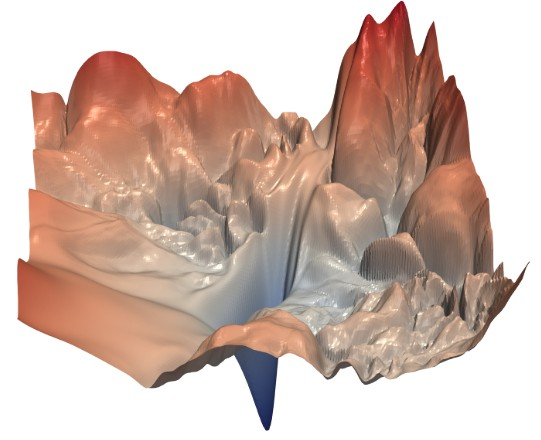
\includegraphics[width=0.8\textwidth]{graphics/Loss_surface_resnet-56.jpg}
                ResNet-56
            \end{column}
            \begin{column}{0.5\textwidth}
                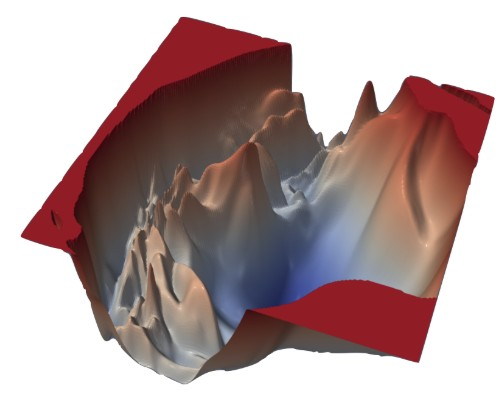
\includegraphics[width=0.8\textwidth]{graphics/Loss_surface_restnet-110.jpg}
                ResNet-110
            \end{column}
        \end{columns}
    \end{frame}

    \begin{frame}
        \frametitle{Background}
        \framesubtitle{The problem with constant learning rates; \cite{zhang2023dive}}
        % recall the parameter update 
        % \begin{align*}
        %     \theta_{t + 1} = \theta_t - \alpha \nabla_{\theta_t} f(\boldsymbol{x}, \theta_t)
        % \end{align*}
        The idea is: a preset constant learning rate throughout the training is not optimal. 
        \begin{itemize}
            \item Too high:  Large jumps, potential for instability and divergence.
            \item Too low: Slow convergence, risk of getting stuck in local minima.
        \end{itemize}
        % This can cause that constant learning rates:
        % \begin{itemize}
        %     \item could be slow in convergence
        %     \item could get stuck in local minima
        % \end{itemize}
    \end{frame}

    \begin{frame}
        \frametitle{Background}
        \framesubtitle{what is a learning rate scheduler?; \cite{zhang2023dive}}
    
        \textbf{Approach}: take the learning parameter $\alpha$ not as a constant but as a function of $t$
        \begin{align*}
            \theta_{t + 1} = \theta_t - \alpha(t) \nabla_{\theta_t} f(\boldsymbol{x}, \theta_t)
        \end{align*}
        With this we try to enable:
        \begin{itemize}
            \item Early rapid exploration with high learning rates.
            \item Finer adjustments and convergence with small learning rates.
            \item Higher stability and avoids getting stuck.
        \end{itemize}
    
    \end{frame}

    \begin{darkframe}
        \frametitle{Outline}
        
        \begin{enumerate}
            \item Background - Why do we schedule learning rates in DL?
            \begin{ribbon}
                \item Which LR schedules are used in practice?
            \end{ribbon}
            \item Experiments
            \item Scheduling other Hyperparameter
            \item Conclusion
        \end{enumerate}
    \end{darkframe}


    \begin{frame}
        \frametitle{Commonly used Learning-Rate Scheudles}   
        \framesubtitle{Function space}     
        \begin{columns}
            \begin{column}{0.5\textwidth}
                We have a whole function space for $\alpha: \mathbb{R} \to \mathbb{R}$\\
                Which functions are reasonable?
            \end{column}
            \begin{column}{0.5\textwidth}
                \includegraphics[width=\textwidth]{../project/figs/standard/function_space.pdf}
            \end{column}
        \end{columns}
        
    
    \end{frame}

    \begin{frame}
        \frametitle{Commonly used Learning-Rate Scheudler}        
        \framesubtitle{ConstantLR Schedule}
        
        \begin{columns}
            \begin{column}{0.5\textwidth}
                constant learning rate over the whole training. 
                \vspace{0.5cm}

                Advantages
                \begin{itemize}
                    \item Trivial implementation
                    \item Useful baseline
                \end{itemize}

                Disadvantages
                \begin{itemize}
                    \item More sensitive to high learning rates
                    \item Has to comprehend for fast exploration and refinement
                \end{itemize}
            \end{column}
            \begin{column}{0.5\textwidth}
                \includegraphics[width=\textwidth]{../project/figs/standard/ConstantLR.pdf}
            \end{column}
        \end{columns}
    \end{frame}

    
    \begin{frame}
        \frametitle{Commonly used Learning-Rate Scheudler}        
        \framesubtitle{StepLR Schedule}
        
        \begin{columns}
            \begin{column}{0.5\textwidth}
                Multiply learning rate by constant factor every $k$ epochs. 
                \vspace{0.5cm}

                Advantages
                \begin{itemize}
                    \item Aggressive initial learning rate
                    \item Smooth decay 
                \end{itemize}

                Disadvantages
                \begin{itemize}
                    \item Potentially overshoots the solution
                    \item Limited adaptability
                \end{itemize}
            \end{column}
            \begin{column}{0.5\textwidth}
                \includegraphics[width=\textwidth]{../project/figs/standard/StepLR.pdf}
            \end{column}
        \end{columns}
    \end{frame}

    
    \begin{frame}
        \frametitle{Commonly used Learning-Rate Scheudler}        
        \framesubtitle{Cosine Annealing Schedule}
        
        \begin{columns}
            \begin{column}{0.5\textwidth}
                Work done by: \cite{loshchilov2016sgdr}
                Follow the first half  of a cosine period 
                \vspace{0.5cm}

                Advantages
                \begin{itemize}
                    \item Reduces the overshot problem
                    \item Smooth decay 
                \end{itemize}

                Disadvantages
                \begin{itemize}
                    \item Potentially slow convergence (not so aggressive lr in the beginning)
                    \item More parameters to tune
                \end{itemize}
            \end{column}
            \begin{column}{0.5\textwidth}
                \includegraphics[width=\textwidth]{../project/figs/standard/CosineAnnealingLR.pdf}
            \end{column}
        \end{columns}
    \end{frame}


    \begin{frame}
        \frametitle{Commonly used Learning-Rate Scheudler}
        \framesubtitle{Warmup Schedules}

        \begin{columns}
            \begin{column}{0.5\textwidth}
                One of the first appearance w.r.t DL in \cite{he2016deep}.

                \begin{enumerate}
                    \item Gradually increasing the learning rate until a maximum 
                    \item Continue with any schedule you like
                \end{enumerate}
                \vspace{0.5cm}
                
                Advantages (\cite{gotmare2018closer}):
                \begin{itemize}
                    \item Lowers the amount of divergence of parameters by the end of training
                    \item More stable training for higher learning rates
                    \item Can improve training
                \end{itemize}

                \vspace{0.5cm}
                But it introduces also new hyperparameter
            \end{column}
            \begin{column}{0.5\textwidth}
                \includegraphics[width=\textwidth]{../project/figs/standard/warumup_?.pdf}
            \end{column}
        \end{columns}    
    \end{frame}

    \begin{frame}
        \frametitle{Commonly used Learning-Rate Scheudler}
        \framesubtitle{OneCycle Schedules}

        \begin{columns}
            \begin{column}{0.5\textwidth}
                Proposed by: \cite{smith2019super}
                \begin{enumerate}
                    \item Gradually increasing the learning rate until a maximum 
                    \item Staying on a plateau for exploration
                    \item Decreasing the learning rate for fine-tuning
                \end{enumerate}
                \vspace{0.5cm}
                
                % Advantages:
                % \begin{itemize}
                %     \item lowers the amount of divergence of parameters by the end of training \cite{gotmare2018closer}
                %     \item more stable training for higher learning rates
                %     \item Can improve training
                % \end{itemize}
                Comes with the same advantages as warmup schedules
            \end{column}
            \begin{column}{0.5\textwidth}
                \includegraphics[width=\textwidth]{../project/figs/standard/OneCycle.pdf}
            \end{column}
        \end{columns}    
    \end{frame}

    \begin{frame}
        \frametitle{Commonly used Learning-Rate Scheudler}
        \framesubtitle{Cyclic Learning Rate Schedules}
        \begin{columns}
            \begin{column}{0.5\textwidth}
                Proposed by: \cite{schaul2013no}, \cite{smith2017cyclical} \\
                oscillate between min and max learning rate. \\
                \vspace{0.5cm}
                
                Advantages
                \begin{itemize}
                    \item Explores broader region
                    \item More flexible 
                    \item Avoiding getting stuck
                \end{itemize}

                Disadvantages
                \begin{itemize}
                    \item More complex to tune
                    \item Slow convergence
                    \item Prone to over-fit
                \end{itemize}
            \end{column}
            \begin{column}{0.5\textwidth}
                \includegraphics[width=\textwidth]{../project/figs/standard/CyclicLR.pdf}
            \end{column}
        \end{columns}
    \end{frame}

    \begin{frame}
        \frametitle{Commonly used Learning-Rate Scheudler}
        \framesubtitle{Cosine Annealing with Warm Restarts}
        \begin{columns}
            \begin{column}{0.5\textwidth}
                Proposed by: \cite{loshchilov2016sgdr} \\
                Cyclical learning rate schedule with cosine as decay.
                \vspace{0.5cm}
                \begin{itemize}
                    \item Single decaying cycle
                    \item Less parameters to tune
                    \item Focuses on smooth learning rate decay
                    \item Works well with an over all decay trend \cite{gotmare2018closer}
                \end{itemize}
            \end{column}
            \begin{column}{0.5\textwidth}
                \includegraphics[width=\textwidth]{../project/figs/standard/CosineAnnealingWarmRestarts.pdf}
            \end{column}
        \end{columns}
    \end{frame}

    \begin{frame}
        \frametitle{Commonly used Learning-Rate Scheudler}
        \framesubtitle{Wrapup}

        Decaying Schedules:
        \begin{itemize}
            \item Step Decay: Periodical exponential decay
            \item Exponential Decay: Continuously differentiable version of step decay 
            \item Cosine Annealing: Reduce learning rate following a cosine curve
            \item Linear Decay: Linear decay
        \end{itemize}
        Option to expand those with warmup \\
        \vspace{0.5cm}
        Cyclic:
        \begin{itemize}
            \item Cyclic Learning Rate: Bouncing between max mal and minimal learning rate
            \item Cosine Annealing with Warm Restarts: Decay with cosine and jump back to maximal learning rate
            \item OneCycle: combines the content of cyclic lr schedules in one cycle
        \end{itemize}

        Others like piecewise constant or something else are also valid
        
        % \begin{columns}
        %     \begin{column}{0.5\textwidth}
        %     \end{column}
        %     \begin{column}{0.5\textwidth}
        %     \end{column}
        % \end{columns}
    \end{frame}

    \begin{darkframe}
        \frametitle{Outline}
        \begin{enumerate}
            \item Background - Why do we schedule learning rates in DL?
            \item Which LR schedules are used in practice?
            \begin{ribbon}
                \item Experiments
            \end{ribbon}
            \item Scheduling other Hyperparameter
            \item Conclusion
        \end{enumerate}
    \end{darkframe}

    \begin{frame}
        \frametitle{Experiments}
        \framesubtitle{Setup}
        \begin{itemize}
            \item Task: Image Classification 
            \item Dataset: CIFAR10 \cite{krizhevsky2009learning}
            \item architecture: small ViT (approx. 12.5M params scaled down version from \cite{dosovitskiy2020image} at \cite{ViTCIFAR})
            \item optimizer: AdamW with weight decay $10^{-4}$ and different learning rates  \cite{loshchilov2017decoupled}
            \item Training for 100 epochs
            \item Batch size: 512 training, 2048 validation and testing
        \end{itemize}
        Metrics:
        \begin{itemize}
            \item Cross Entropy
            \item Accuracy
            \item Test best model w.r.t. validation accuary
        \end{itemize}
        Various configured learning rate scheduler
        % Scheduler:
        % \begin{itemize}
        %     \item ConstantLR (warmup)			
        %     \item CosineAnnealingLR (warmup)
        %     \item StepLR
        %     \item CosineAnnealingWarmRestarts
        %     \item OneCycleLR
        % \end{itemize}
    \end{frame}
    
    \begin{frame}
        \frametitle{Experiments}
        \framesubtitle{Scheduler Search Space}
        \begin{center}
            \begin{tabular}{l||l|l}
                Scheduler & Parameter & Search Space \\
                \hline\hline
                ConstantLR (warmup)         & factor = 1, *                                 & lr $\in [10^{-6}, 10^{-2}]$\\
                CosineAnnealingLR (warmup)  & $T_{\max} = 100$, $\eta_{\min} = 10^{-6}$, *  & lr $\in [10^{-5}, 10^{-2}]$\\
                StepLR                      & step size = 5, $\gamma = 0.9$                 & lr $\in [10^{-5}, 10^{-2}]$\\
                OneCycleLR                  & total steps = 100                             & max\textunderscore lr  $\in [10^{-5}, 10^{-2}]$ \\
                CosineAnnealingWarmRestarts & lr $ \approx 4.6 \cdot 10^{-4}$               & $T_0 \in [10, 50]$\\
            \end{tabular} \\
        \end{center}
        *: for the warmup version we choose 6 warmup epochs
    \end{frame}


    \begin{frame}
        \frametitle{Experiments}
        \framesubtitle{Test Accuracy}
        \begin{columns}
            \begin{column}{0.5\textwidth}
                Test accuracy per deployed learning rate factor
                \begin{itemize}
                    \item While increasing the maximal learning rate, predictor performance varies across different schedules
                    \item But we can spot similarities between schedules
                \end{itemize}
            \end{column}
            \begin{column}{0.5\textwidth}
                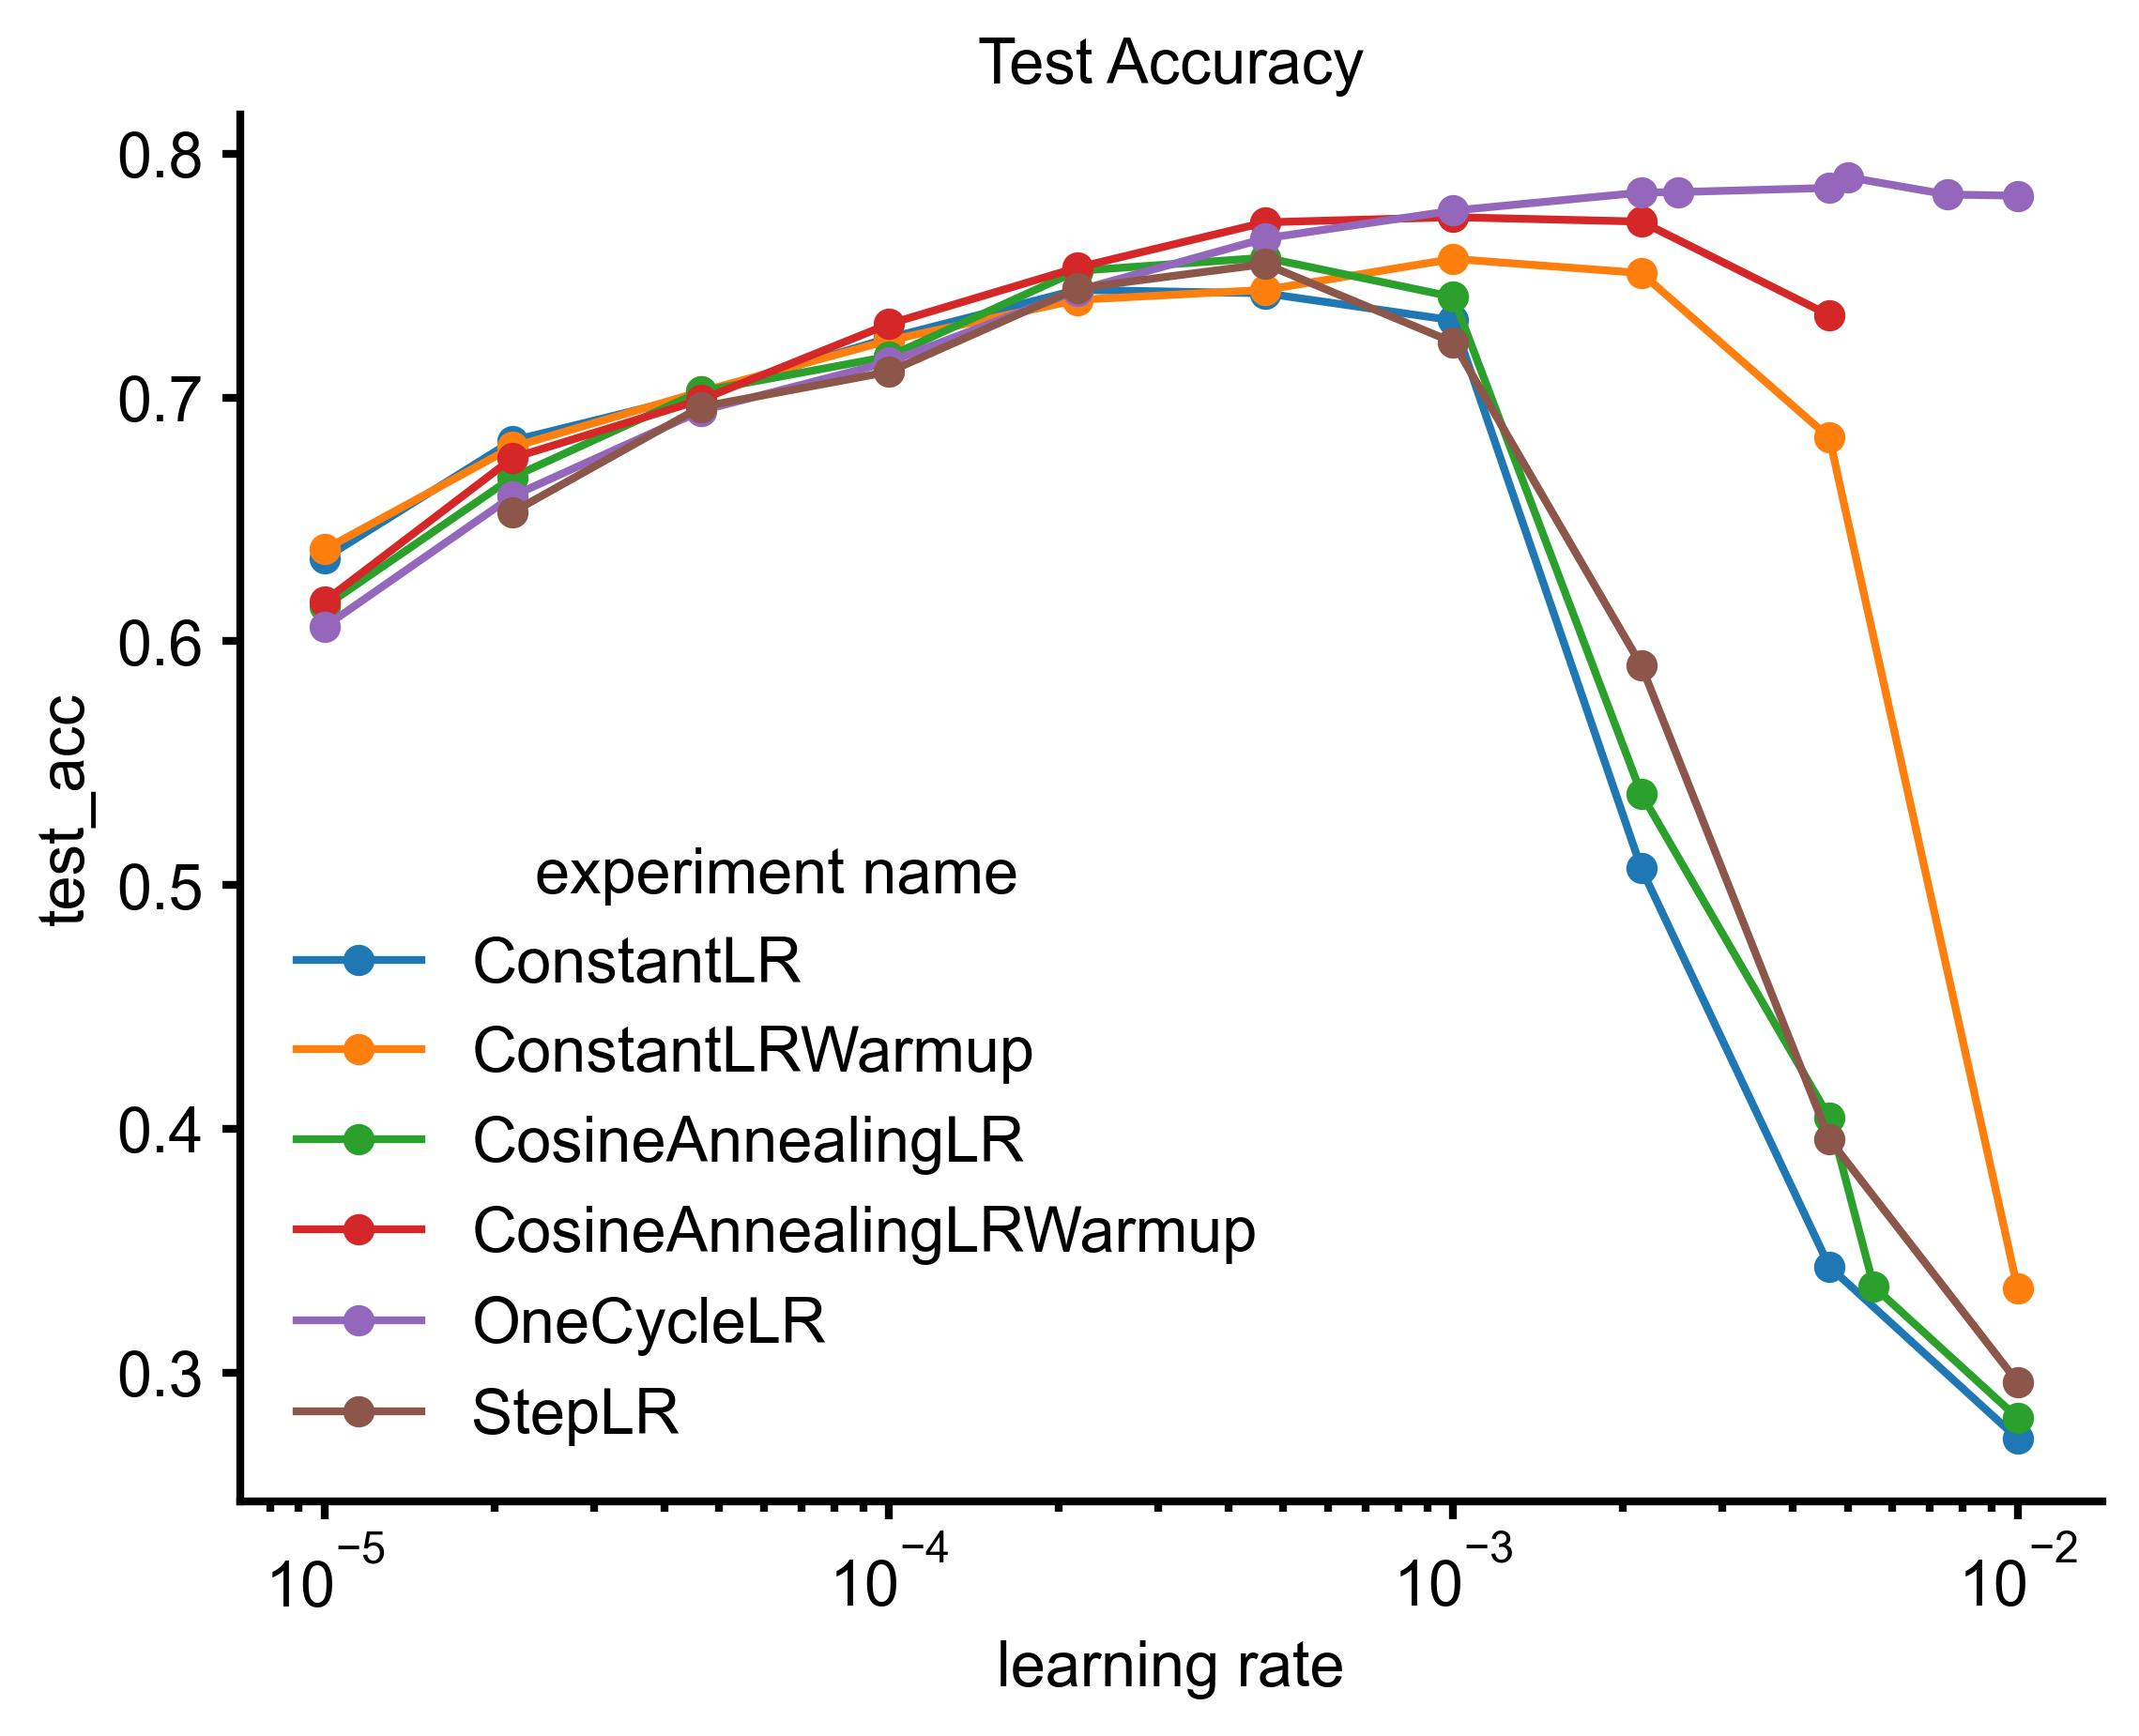
\includegraphics[width=\textwidth]{../project/figs/test_acc_scatter.pdf}
            \end{column}
        \end{columns}
    \end{frame}
    

    \begin{frame}
        \frametitle{Experiments}
        \framesubtitle{Test Accuracy Groups}
        \begin{columns}
            \begin{column}{0.5\textwidth}
                OneCycle Learning Rate:
                \begin{itemize}
                    \item Seems to work best in the current setup 
                    \item Able to handle high maximal learning rate 
                \end{itemize}
                Purly Decaying / Constant
                \begin{itemize}
                    \item Similar to OneCycle for small learning rates
                    \item Begin to diverge very early
                \end{itemize}
                Warmup Schedules: \\ (ConstantLR and CosineAnnealingLR with Warmup)
                \begin{itemize}
                    \item Seems to produce slightly better results
                    \item Makes training more stable
                \end{itemize}
            \end{column}
            \begin{column}{0.5\textwidth}
                \includegraphics[width=\textwidth]{../project/figs/test_accuracy_group_fit.pdf}
            \end{column}
        \end{columns}
    \end{frame}

    \begin{frame}
        \frametitle{Experiments}
        \framesubtitle{Influence of Warmup}
        \begin{columns}
            \begin{column}{0.5\textwidth}
                \includegraphics[width=\textwidth]{../project/figs/ConstantLR_val_warmup.pdf}
                Constant Learning Rate
            \end{column}
            \begin{column}{0.5\textwidth}
                \includegraphics[width=\textwidth]{../project/figs/CosineAnnealingLR_val_warmup.pdf}
                Cosine Annealing
            \end{column}
        \end{columns}
    \end{frame}
    
    \begin{frame}
        \frametitle{Experiments}
        \framesubtitle{Convergence / Divergence}
        \begin{columns}
            \begin{column}{0.5\textwidth}
                At which epoch was the model at its best and how high was the learning rate?

                \begin{itemize}
                    \item Convergence region (upper right): smooth gradient towards maximal accuracy late in the training process 
                    \item Divergence / under-fit region (lower left): high learning rates and low accuracy early in training
                \end{itemize}
            \end{column}
            \begin{column}{0.5\textwidth}
                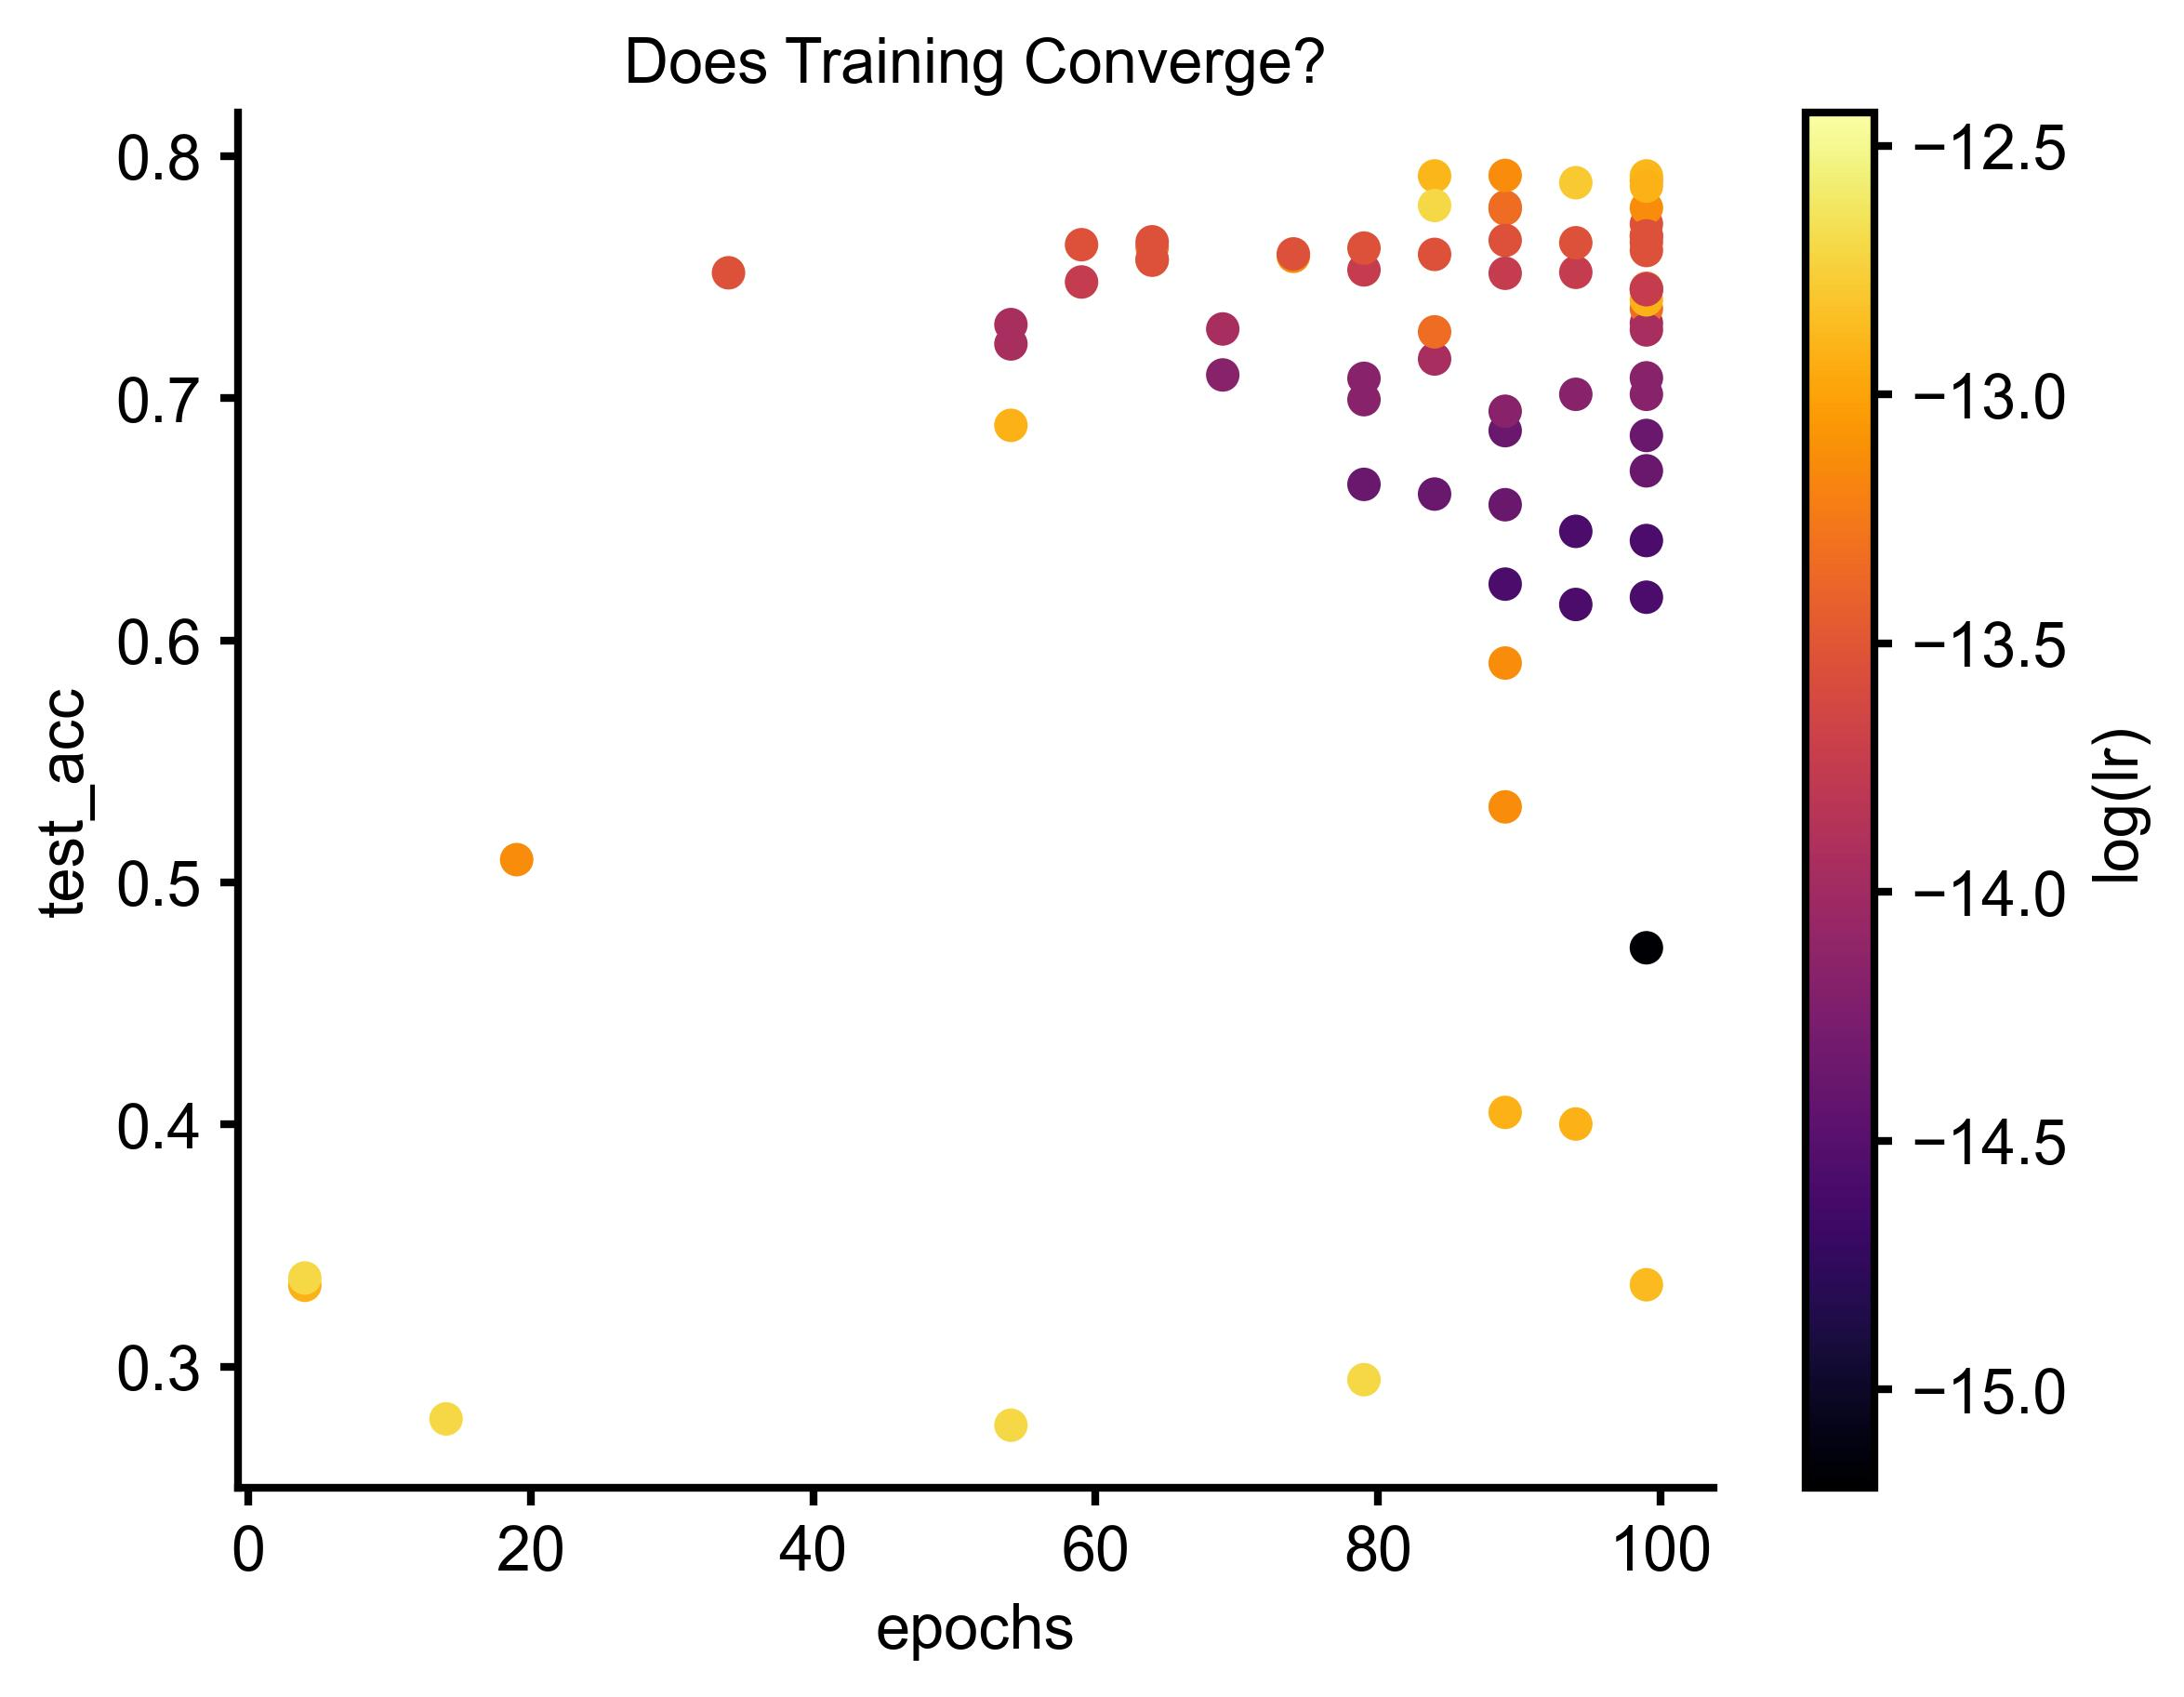
\includegraphics[width=\textwidth]{../project/figs/Convergence_Divergence.pdf}
            \end{column}
        \end{columns}
    \end{frame}

    \begin{frame}
        \frametitle{Experiments}
        \framesubtitle{Convergence / Divergence}
        \begin{columns}
            \begin{column}{0.5\textwidth}
                At which epoch was the model at its best and how high was the learning rate?
                \begin{itemize}
                    \item Convergence region (upper right): smooth gradient towards maximal accuracy late in the training process 
                    \item Divergence / under-fit region (lower left): high learning rates and low accuracy early in training
                \end{itemize}
            \end{column}
            \begin{column}{0.5\textwidth}
                \includegraphics[width=\textwidth]{../project/figs/Convergence_Divergence_scheduler.pdf}
            \end{column}
        \end{columns}
    \end{frame}

    \begin{frame}
        \frametitle{Experiments}
        \framesubtitle{Limitations}
        Setup
        \begin{itemize}
            \item Dataset size. Other datasets might reveal a higher variance in training behavior
            \item Model Complexity: The simplified ViT could be not as sensitive as large scale models
        \end{itemize}
        \vspace{0.5cm}
        Training
        \begin{itemize}
            \item Limited exploration space
            \item Tuning only for scheduler hyperparameter, leaving other parameters constant
            \item Training duration
            \item Used metrics could be expanded also F1 score, … 
            \item No statistical significance conducted. 
        \end{itemize}
    \end{frame}


    \begin{darkframe}
        \frametitle{Outline}
        \begin{enumerate}
            \item Background - Why do we schedule learning rates in DL?
            \item Which LR schedules are used in practice?
            \item Experiments
            \begin{ribbon}
                \item Scheduling other Hyperparameter
            \end{ribbon}
            \item Conclusion
        \end{enumerate}
    \end{darkframe}

    \begin{frame}
        \frametitle{Scheduling other Hyperparameter}
        \framesubtitle{Overview}
        Learning rate is not the only hyperparameter that benefits from scheduling.
        Benefits:
        \begin{itemize}
            \item Fine-tuning hyperparameter values throughout training can lead to better performance and stability.
            \item Allows for more sophisticated training strategies that adapt to the learning process.
        \end{itemize}

        \vspace{0.5cm}
        Exmaples of current research schedules 3 other parameter:
        \begin{itemize}
            \item Batch Size: \cite{smith2017don}
            \item Momentum: \cite{sun2021training}
            \item Weight Decacy: \cite{xie2024overlooked}
        \end{itemize}
        But you can basically schedule everything you want. 
    \end{frame}

    \begin{frame}
        \frametitle{Scheduling other Hyperparameter}
        \framesubtitle{Batch Size}
        Work done by: \cite{smith2017don}\\
        \vspace{0.5cm}
        Instead of increasing the learning rate they propose to increase the batch-size. 
        \begin{itemize}
            \item More accurate estimate of the true gradient
            \item Update step size is proportional to both the learning rate and the batch size $\to$ batch size effectively reduces the learning rate
        \end{itemize}
        \vspace{0.5cm}
        Advantages
        \begin{itemize}
            \item Reduced the number of parameter-updates required
            \item Their scaling rules enable them to use existing hyperparameter-configurations
        \end{itemize}
    \end{frame}

    \begin{frame}
        \frametitle{Scheduling other Hyperparameter}
        \framesubtitle{Momentum}
        Work done by \cite{sun2021training} \\
        \vspace{0.5cm}
        \textbf{Problem}: Momentum $\beta$ as fixed hyperparameter. Setting it could be quite challenging \\
        \begin{align*}
            \theta_{t +1 } = \theta_t - \alpha \nabla_{\theta_t} f(\boldsymbol{x}; \theta_t) + \beta (\theta_t - \theta_{t - 1})
        \end{align*}
        
        \textbf{Solution}: Adaptive heavy ball momentum (Polyak momentum), inspired by the optimal choice of momentum for quadratic optimization problems. Adjusts automatically based on past gradients $\to$ no manual tuning needed
        \vspace{0.5cm}
        Advantages:
        \begin{itemize}
            \item Convergences faster than those with fixed momentum.
            \item More robust w.r.t. large learning rates
            \item Might generalize better to unseen data.
        \end{itemize}
    \end{frame}

    \begin{frame}
        \frametitle{Scheduling other Hyperparameter}
        \framesubtitle{Weight Decay}
        Work done by: \cite{xie2024overlooked}\\
        \vspace{0.5cm}
        \textbf{Problem}: Weight decay is a regularization technique, helps prevent over-fitting. But large weight decay can lead to large gradient norms during the final stages of training. This could lead to:
        Destabilize training, Hinder convergence\\ 
        \textbf{Solution}: Paper proposes Scheduled-Weight-Decay (SWD), dynamically adjusts the weight decay strength based on the gradient norm.
        \begin{itemize}
            \item High Gradient Norm - Lower Weight Decay
            \item Low Gradient Norm - Higher Weight Decay
        \end{itemize}
        This feedback loop leads to:
        \begin{itemize}
            \item Simpler Hyperparameter Tuning
            \item Improved Convergence
            \item Better Generalization
        \end{itemize}
    \end{frame}

    \begin{darkframe}
        \frametitle{Outline}
        \begin{enumerate}
            \item Background - Why do we schedule learning rates in DL?
            \item Which LR schedules are used in practice?
            \item Experiments
            \item Scheduling other Hyperparameter
            \begin{ribbon}
                \item Conclusion
            \end{ribbon}
        \end{enumerate}
    \end{darkframe}

    \begin{frame}
        \frametitle{Conclusion}
        \begin{itemize}
            \item Learning rate scheduler are a reasonable aspect in improving training neural networks
            \begin{itemize}
                \item They can speed up training
                \item Find better optima
                \item Stabilize training
            \end{itemize}
            \item But the also open up a huge parameter space to optimize.
            \item Tuning one schedule does not mean we can map those result on any other schedule.
            \item There is no single 'best' schedule for every model.
            \item Scheduling other parameters could be use-full for boosting performance. But still come at the cost of tuning additional parameters. 
        \end{itemize}
        
    
    \end{frame}

    \begin{frame}[allowframebreaks]
        \frametitle{References}
        % \bibliography{./bibliography.bib}
        % \bibliographystyle{ieee}
        \printbibliography        
    \end{frame}


    \begin{frame}
        \frametitle{Thank you for your attention}
        \begin{columns}
            \begin{column}{0.7\textwidth}
                {\Huge Thank you for your attention.} \\
                \vspace{1cm}
                {\huge Questions?} \\
                \vspace{1cm}
                GitHub: https://github.com/RobinU434/DeepLearningResearchKitchen.git
            \end{column}
            \begin{column}{0.3\textwidth}
                \begin{center}
                    
\includegraphics[width=\textwidth]{graphics/Repo_code.jpg}
                \end{center}
            \end{column}
        \end{columns}
    \end{frame}

    \blackslide

    \begin{frame}
        \frametitle{Appendix}
        \begin{columns}
            \begin{column}{0.5\textwidth}
                \includegraphics[width=\textwidth]{../project/figs/ConstantLR_train.pdf}
            \end{column}
            \begin{column}{0.5\textwidth}
                \includegraphics[width=\textwidth]{../project/figs/ConstantLR_val.pdf}
            \end{column}
        \end{columns}
    
    \end{frame}

    \begin{frame}
        \frametitle{Appendix}
        \begin{columns}
            \begin{column}{0.5\textwidth}
                \includegraphics[width=\textwidth]{../project/figs/CosineAnnealingLR_train.pdf}
            \end{column}
            \begin{column}{0.5\textwidth}
                \includegraphics[width=\textwidth]{../project/figs/CosineAnnealingLR_val.pdf}
            \end{column}
        \end{columns}
    
    \end{frame}


    \begin{frame}
        \frametitle{Appendix}
        \begin{columns}
            \begin{column}{0.5\textwidth}
                \includegraphics[width=\textwidth]{../project/figs/StepLR_train.pdf}
            \end{column}
            \begin{column}{0.5\textwidth}
                \includegraphics[width=\textwidth]{../project/figs/StepLR_val.pdf}
            \end{column}
        \end{columns}
    
    \end{frame}

    \begin{frame}
        \frametitle{Appendix}
        \begin{columns}
            \begin{column}{0.5\textwidth}
                \includegraphics[width=\textwidth]{../project/figs/OneCycleLR_train.pdf}
            \end{column}
            \begin{column}{0.5\textwidth}
                \includegraphics[width=\textwidth]{../project/figs/OneCycleLR_val.pdf}
            \end{column}
        \end{columns}
    
    \end{frame}

    \begin{frame}
        \frametitle{Appendix}
        \begin{columns}
            \begin{column}{0.5\textwidth}
                \includegraphics[width=\textwidth]{../project/figs/CosineAnnealingWarmRestarts_train.pdf}
            \end{column}
            \begin{column}{0.5\textwidth}
                \includegraphics[width=\textwidth]{../project/figs/CosineAnnealingWarmRestarts_val.pdf}
            \end{column}
        \end{columns}
    
    \end{frame}



    \begin{frame}
        \frametitle{Appendix}
        \framesubtitle{Heavy Ball Momentum update}
        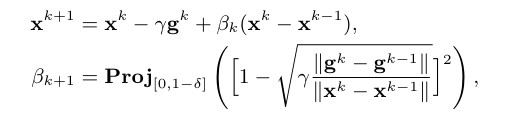
\includegraphics{graphics/heavy_ball_momentum_update.jpg}
    \end{frame}


    \begin{frame}
        \frametitle{Appendix}
        \framesubtitle{Infinite Learning Rate Schedules}
        When your training budget is infinite you can follow approaches like:
        \begin{itemize}
            \item Cyclical Learning Rates (CLR) for Long-Range Optimization: multiple cycles of increasing and decreasing the learning rate, allowing the model to explore a wider range of learning rates and potentially avoid getting stuck in local minima.
            \item AutoLRS: Automatic Learning-Rate Schedule by Bayesian Optimization on the Fly \cite{jin2021autolrs}
        \end{itemize}
    \end{frame}
    \blackslide
    

    % \begin{frame}{Test}
    %     \frametitle{Itemizations, Enumerations, and Descriptions}
    %     \framesubtitle{Itemizations and Enumerations}
    %     %
    %     There are three important points:
    %     %
    %     \begin{enumerate}
    %         \item A first one,
    %         \item a second one with a bunch of subpoints,
    %             \begin{itemize}
    %                 \item first subpoint.
    %                 \item second subpoint.
    %                 \item third subpoint.
    %             \end{itemize}
    %         \item and a third one.
    %     \end{enumerate}
    % \end{frame}
% 
% 
    % \begin{frame}
    %     \frametitle{Itemizations, Enumerations, and Descriptions}
    %     \framesubtitle{Descriptions}
    %     %
    %     \EastGradPerson{graphics/flowlines_dark.png}{Flow Lines}
    %     %
    %     \begin{description}[longest label]
    %         \item[short] Some text.
    %         \item[longest label] Some text.
    %         \item[long label] Some text.
    %     \end{description}
    % \end{frame}
% 
    % \begin{frame}
    %     \frametitle{Block Environments}
    %     %
    %     \begin{block}{Block}
    %         A \alert{regular} block.
    %     \end{block}
    %     %
    %     \begin{alertblock}{Alerted Block}
    %         An \alert{alerted} block.
    %     \end{alertblock}
    %     %
    %     \begin{exampleblock}{Example Block}
    %         An \alert{example} block.
    %     \end{exampleblock}
    % \end{frame}
% 
    % \begin{frame}
    %     \frametitle{Theorem Environments}
    %     \framesubtitle{Theorems and Proofs \hfill Test}
    %     %
    %     \begin{theorem}
    %         There is \alert{no largest} prime number.
    %     \end{theorem}
    %     %
    %     \begin{proof}
    %         \begin{enumerate}
    %             \item<1-| alert@1> Suppose $p$ were the largest prime number.
    %             \item<2-> Let $q$ be the product of the first $p$ numbers.
    %             \item<3-> Then $q+1$ is not divisible by any of them.
    %             \item<1-> But $q + 1$ is greater than $1$, thus divisible by some
    %                 prime
    %                 number not in the first $p$ numbers.
    %         \end{enumerate}
    %     \end{proof}
    % \end{frame}
% 
    % \begin{frame}
    %     \frametitle{Ribbons}
    %     %
    %     \begin{ribbon}
    %         There are three \alert{important} points:
    %         %
    %         \begin{enumerate}
    %             \item A first one,
    %             \item a second one with a bunch of subpoints,
    %                 \begin{itemize}
    %                     \item first subpoint.
    %                     \item second subpoint.
    %                     \item third subpoint.
    %                 \end{itemize}
    %             \item and a third one.
    %         \end{enumerate}
    %     \end{ribbon}
    % \end{frame}

    % \begin{darkframe}
    %     \frametitle{Dark Frames}
    %     %
    %     Normal Text
    %     %
    %     \begin{ribbon}
    %         Ribbon \alert{Alert}
    %         %
    %         \begin{itemize}
    %             \item ItemiBze
    %         \end{itemize}
    %         %
    %         \begin{enumerate}
    %             \item Enumerate
    %         \end{enumerate}
    %     \end{ribbon}
    %     %
    %     Normal Text
    % \end{darkframe}

    % \blackslide
\end{document}
